\tikzset{every picture/.style={line width=0.75pt}} %set default line width to 0.75pt        
\begin{center}
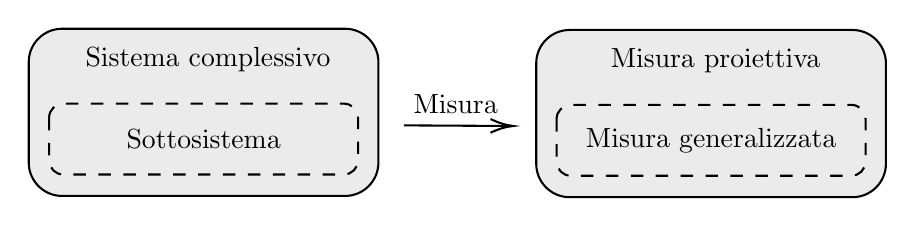
\begin{tikzpicture}[x=0.75pt,y=0.75pt,yscale=-1,xscale=1]
%uncomment if require: \path (0,300); %set diagram left start at 0, and has height of 300

%Rounded Rect [id:dp6106726008236387] 
\draw  [color={rgb, 255:red, 0; green, 0; blue, 0 }  ,draw opacity=1 ][fill={rgb, 255:red, 194; green, 194; blue, 194 }  ,fill opacity=0.33 ] (359.01,102.71) .. controls (359.01,93.81) and (366.22,86.6) .. (375.12,86.6) -- (511.39,86.6) .. controls (520.29,86.6) and (527.5,93.81) .. (527.5,102.71) -- (527.5,151.05) .. controls (527.5,159.95) and (520.29,167.17) .. (511.39,167.17) -- (375.12,167.17) .. controls (366.22,167.17) and (359.01,159.95) .. (359.01,151.05) -- cycle ;
%Rounded Rect [id:dp8954205367068233] 
\draw  [dash pattern={on 4.5pt off 4.5pt}] (368.83,129.52) .. controls (368.83,125.75) and (371.89,122.69) .. (375.66,122.69) -- (510.85,122.69) .. controls (514.62,122.69) and (517.68,125.75) .. (517.68,129.52) -- (517.68,150) .. controls (517.68,153.78) and (514.62,156.83) .. (510.85,156.83) -- (375.66,156.83) .. controls (371.89,156.83) and (368.83,153.78) .. (368.83,150) -- cycle ;
%Rounded Rect [id:dp5246313063373345] 
\draw  [color={rgb, 255:red, 0; green, 0; blue, 0 }  ,draw opacity=1 ][fill={rgb, 255:red, 194; green, 194; blue, 194 }  ,fill opacity=0.33 ] (114.5,102.11) .. controls (114.5,93.21) and (121.71,86) .. (130.61,86) -- (266.88,86) .. controls (275.78,86) and (282.99,93.21) .. (282.99,102.11) -- (282.99,150.45) .. controls (282.99,159.35) and (275.78,166.57) .. (266.88,166.57) -- (130.61,166.57) .. controls (121.71,166.57) and (114.5,159.35) .. (114.5,150.45) -- cycle ;
%Rounded Rect [id:dp909540949537371] 
\draw  [dash pattern={on 4.5pt off 4.5pt}] (124.32,128.92) .. controls (124.32,125.15) and (127.38,122.09) .. (131.15,122.09) -- (266.34,122.09) .. controls (270.11,122.09) and (273.17,125.15) .. (273.17,128.92) -- (273.17,149.41) .. controls (273.17,153.18) and (270.11,156.23) .. (266.34,156.23) -- (131.15,156.23) .. controls (127.38,156.23) and (124.32,153.18) .. (124.32,149.41) -- cycle ;
%Straight Lines [id:da4759430012113268] 
\draw    (295.23,132.57) -- (345.94,132.86) ;
\draw [shift={(347.94,132.87)}, rotate = 180.33] [color={rgb, 255:red, 0; green, 0; blue, 0 }  ][line width=0.75]    (10.93,-3.29) .. controls (6.95,-1.4) and (3.31,-0.3) .. (0,0) .. controls (3.31,0.3) and (6.95,1.4) .. (10.93,3.29)   ;


% Text Node
\draw (445.4,101.27) node  [align=left] {Misura proiettiva};
% Text Node
\draw (443.25,139.76) node  [align=left] {Misura generalizzata};
% Text Node
\draw (200.89,100.68) node  [align=left] {Sistema complessivo};
% Text Node
\draw (198.75,139.16) node  [align=left] {Sottosistema};
% Text Node
\draw (320.18,122.09) node  [align=left] {Misura};


\end{tikzpicture}
\end{center}